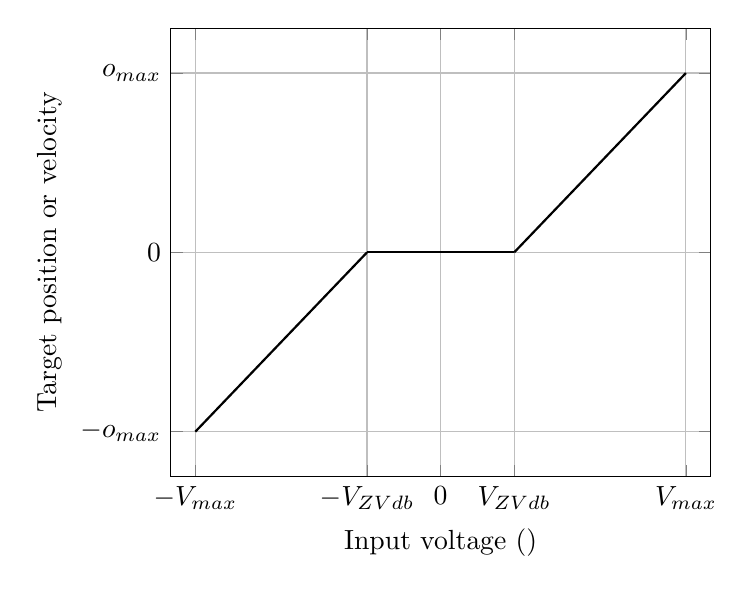
\begin{tikzpicture}
    \def\VMax{10}
    \def\VDeadBand{3}
    
    \begin{axis}[
        % height=6cm,
        % width=10cm,
        xlabel={Input voltage (\unit{\V})},
        ylabel={Target position or velocity},
        xmin=-11,
        xmax=11,
        ymin=-1.25,
        ymax=1.25,
        xtick={-\VMax, -\VDeadBand, 0, \VDeadBand, \VMax},
        xticklabels={
            $-V_{\text{max}}$,
            $-V_{\text{ZVdb}}$,
            0,
            $V_{\text{ZVdb}}$,
            $V_{\text{max}}$
        },
        ytick={-1, 0, 1},
        yticklabels={$-o_{\text{max}}$, 0, $o_{\text{max}}$},
        grid=both,
    ]
    % Recta 1
    \addplot [domain=-\VMax:-\VDeadBand, thick] {(x + \VDeadBand)/(\VMax - \VDeadBand)};

    % Recta 2
    \addplot [domain=-\VDeadBand:\VDeadBand, thick] {0};

    % Recta 3
    \addplot [domain=\VDeadBand:\VMax, thick] {(x - \VDeadBand)/(\VMax - \VDeadBand)};
    
    \end{axis}
\end{tikzpicture}